\documentclass[a4paper,10pt]{article}
\usepackage[paper=a4paper,top=2.5cm,bottom=2.5cm,left=2.5cm,right=2.5cm,bottom=2.5cm,foot=1cm]{geometry}

\usepackage{chngpage}
\usepackage{graphicx}
\usepackage[T1]{fontenc}
\usepackage{lmodern}
\usepackage[usenames,dvipsnames]{color}
\usepackage{hyperref}
\usepackage{url}
\usepackage{pdfpages}
\usepackage{float}
\usepackage{array}
\usepackage{verbatim}
\usepackage{enumitem}
\usepackage{fancyhdr}

\pagestyle{headings}

%% -- document formating -- begin -- %%
\makeatletter				% section title formating
\renewcommand\section{\@startsection {section}{1}{\z@}%
                   {-3.5ex \@plus -1ex \@minus -.2ex}%
                   {2.3ex \@plus.2ex}%
                   {\normalfont\sffamily\Large\bfseries\color{BrickRed}}}
\renewcommand\subsection{\@startsection{subsection}{2}{\z@}%
                   {-3.25ex\@plus -1ex \@minus -.2ex}%
                   {1.5ex \@plus .2ex}%
                   {\normalfont\sffamily\large\bfseries\color{BrickRed}}}
\renewcommand\subsubsection{\@startsection{subsubsection}{3}{\z@}%
                   {-3.25ex\@plus -1ex \@minus -.2ex}%
                   {1.5ex \@plus .2ex}%
                   {\normalfont\normalsize\sffamily\bfseries\color{BrickRed}}}
\makeatother

\newenvironment{itemize*}%
{\begin{itemize}%
    \setlength{\itemsep}{0pt}%
    \setlength{\parskip}{0pt}%
}{\end{itemize}}

% ----- The next line is important when dealing with alpha channels
% see http://bmeps.sourceforge.net/examples.html
\pdfpageattr {/Group << /S /Transparency /I true /CS /DeviceRGB>>}

%% -- document formating -- end -- %%

\renewcommand{\headrulewidth}{0pt}
\fancyhead[L]{\sffamily\footnotesize User Manual}
\fancyhead[C]{}
\fancyhead[R]{\sffamily\footnotesize SSHCure -- A Flow-Based SSH Intrusion Detection System}
\fancyfoot[L]{\sffamily\footnotesize Rick Hofstede, Luuk Hendriks}
\fancyfoot[C]{}
\fancyfoot[R]{\sffamily\footnotesize Page \thepage/\pageref{totalpages}}

\begin{document}

% Title Page
\pdfbookmark[1]{Title Page}{pdf_first_page}
\pagestyle{empty}
\sffamily\Large

\begin{center}
	\vspace*{1cm} 
\includegraphics[width=0.7\linewidth]{img/UT_Logo_Black_RGB_EN}

%	\vspace{4cm} {\fontsize{60pt}{80pt}\selectfont\bfseries\color{BrickRed} SSHCure}
	\vspace{3cm}
	\begin{figure}[!h]
		\centering
		
\includegraphics[width=0.75\textwidth]{img/sshcure_logo.png}
	\end{figure}

	\vspace{4cm} {\Huge\bfseries A Flow-Based SSH \\[0.3cm] Intrusion Detection System}

	\vspace{1cm} {\LARGE\bfseries User Manual}
\end{center}

\vspace{3cm}

\begin{tabular}{rl}
	\bfseries Author & Rick Hofstede, Luuk Hendriks \\
	 & \\
	\bfseries Address &  University of Twente, The Netherlands \\
	 & \\
	\bfseries Date & \today \\
	 & \\
	\bfseries Version & 3.0
\end{tabular}

\cleardoublepage

\pdfbookmark[1]{Contents}{pdf_contents}            % link to Contents in pdf bookmarks
\label{pdf_contents}
\pagestyle{fancy}

\normalsize
\tableofcontents

\newpage\cleardoublepage\normalfont

\section{Introduction}
\label{sec:introduction}

SSHCure is a flow-based SSH intrusion detection system (IDS). As a plugin for the state-of-the-art flow collector NfSen \cite{nfsen}, it supports and processes any NetFlow \cite{rfc3954} and IPFIX \cite{rfc5470}. sFlow \cite{sflowv5} is currently not supported, as it is not a flow export technology. The core of SSHCure is an algorithm based on the work of Sperotto \textit{et al}., who identify and classify SSH-based dictionary attacks in three phases \cite{sperotto2009}:

\begin{enumerate}
	\item \textbf{Scan phase} -- This is usually the first phase of an SSH attack, where an attacker performs a horizontal scan over a certain IP address range.
	
	\item \textbf{Brute-force phase} -- Either immediately following the scan phase or at a later point in time, an attacker may try to login to a certain host on which it found to have a running SSH daemon. It does so by generating username/password combinations at a usually very high speed.
	
	\item \textbf{Die-off phase} -- The last phase of a dictionary attack represents the situation in which the brute-force phase has been successful for the attacker and the attacker managed to login to the target machine. From that moment the time, the target machine has been compromised and is under attacker control.
\end{enumerate}

SSHCure consists of both a backend that runs the actual IDS and a frontend that aims to give operators and Computer Emergency Response Teams (CERTs) insight into the current state of their networks. This is done by means of several levels: The \textit{Dashboard} gives an overview of attacks, top attackers/targets, etc. for a selected period of time. More details about a selected attack can be obtained from the \textit{Attack Details} page, where a profile of the attack is shown, together with a target overview and the option to analyse the related flow data. Finally, the \textit{Host Details} page shows in which attacks a certain host has participated, either in the role of attacker or target.

SSHCure has been optimized and tested for use in Mozilla FireFox (3+), Apple Safari (4+) and Google Chrome (12+). The SSHCure source code (and this manual) will always be made available through the SSHCure project's Web page on GitHub. This page is reachable by the following URLs:

\begin{itemize}
	\item SSHCure project main page: \url{https://github.com/sshcure/sshcure}
	\item SSHCure project download link: \url{https://github.com/SSHCure/SSHCure/archive/master.zip}
\end{itemize}

The work on SSHCure has been supported by the following publication(s):

\begin{enumerate}
	\item Rick Hofstede, Luuk Hendriks, Anna Sperotto, Aiko Pras. \textit{SSH Compromise Detection using NetFlow/IPFIX}. In: ACM SIGCOMM Computer Communication Review, Vol. 44, No. 5, 2014, ISSN 0146-4833, pp. 20--26
	
	\item Laurens Hellemons, Luuk Hendriks, Rick Hofstede, Anna Sperotto, Ramin Sadre, Aiko Pras. \textit{SSHCure: A Flow-Based SSH Intrusion Detection System}. In: Dependable Networks and Services. Proceedings of the 6th International Conference on Autonomous Infrastructure, Management and Security (AIMS 2012), 4-8 June 2012, Luxembourg, Luxembourg. Lecture Notes in Computer Science, Vol. 7279, ISSN 0302-9743 ISBN 978-3-642-30632-7, pp. 86-97
\end{enumerate}

The following chapters cover details on the installation and configuration of SSHCure. In particular, Chapter~\ref{sec:installation} includes details on the installation that have been omitted in the readme file. Details on the configuration, combined with best practices, are included in Chapter~\ref{sec:configuration}. After that, Chapter~\ref{sec:using_sshcure} outlines how to use SSHCure. The last chapter of this manual, Chapter~\ref{sec:troubleshooting_faq} explains what to do in case of any problem and discusses some frequently asked questions.
 \newpage
\section{Installation} \label{sec:installation}

This chapter outlines details on the installation of SSHCure, which have not been included in the readme file (\emph{readme.txt}). We refer to this file for the regular installation instructions.

\subsection{Installation Requirements} \label{subsec:installation_requirements}

In order to achieve the best experience when using SSHCure, the following components should be installed:

\begin{itemize}
	\item NfSen
	\item Perl, together with the following modules: DBD SQLite, IP::Net, JSON, LWP
	\item PHP 5.2.4 or newer, together with the following modules: \textit{mbstring}, \textit{PDO SQLite3}
\end{itemize}

These requirements translate to the following packages:

\begin{table}[!h]
	\renewcommand{\arraystretch}{1.3}
	\centering
	\begin{tabular}{r || c | c | c}
									&	\textbf{Debian/Ubuntu}		&	\textbf{RHEL/CentOS} 	&	\textbf{FreeBSD} \\ \hline \hline
		PHP \textit{mbstring} module		&							&	\texttt{php-mbstring} 		&	\texttt{} \\ \hline
		PHP \textit{PDO SQLite3} module	&	\texttt{php5-sqlite}			&	\texttt{php-pdo} 		&	\texttt{} \\ \hline
		Perl DBD SQLite module			&	\texttt{libdbd-sqlite3-perl}		&	\texttt{perl-DBD-SQLite}	&	\texttt{p5-DBD-SQLite} \\ \hline
		Perl IP::Net module				& 	\texttt{libnet-ip-perl}			&	\texttt{perl-Net-IP} 		&	\texttt{p5-Net-IP} \\ \hline
		Perl JSON module				& 	\texttt{libjson-perl}			&	\texttt{perl-JSON} 		&	\texttt{p5-JSON} \\ \hline
		Perl LWP module				&	\texttt{libwww-perl}			&	\texttt{perl-libwww-perl} 	&	\texttt{p5-libwww} \\ \hline
	\end{tabular}
\end{table}
 \newpage
\section{Configuration} \label{sec:configuration}

In most setups it will suffice to configure SSHCure in the backend, leaving the frontend configuration untouched. This chapter will therefore first describe the configuration in the backend in Chapter~\ref{subsec:backend_configuration}, followed by the frontend configuration in Chapter~\ref{subsec:frontend_configuration}.

\subsection{Backend} \label{subsec:backend_configuration}

All backend configuration options discussed in this section can be found in the backend configuration file \textit{config.pm}.

\subsubsection{NfSen sources}

Many NfSen-based flow collectors receive flow data from multiple flow exporters. By default, SSHCure considers the flow data from all available sources for its processing. This may, however, not yield the optimal setup and detection results for two reasons:

\begin{enumerate}
	\item Flows may pass multiple observation points, which will result in multiple records for the same flow. This interferes with the detection algorithms of SSHCure.
	\item Processing times increase as more data is used for processing.
\end{enumerate}

As a best-practice, you should use only ingress/egress flow data from your edge routers/links. This can be accomplished by configuring the name of the desired data sources in the file \textit{config.pm}. The appropriate setting name is OVERRIDE\_SOURCE, which can contain one or more source names. For example, if two sources named \textit{router1} and \textit{router2} should be used by SSHCure, you can configure it as follows: \\

OVERRIDE\_SOURCE = ``router1:router2'' \hfill (note the colon for separating the names) \\

SSHCure's frontend will automatically use this setting as well, when retrieving flow records from the backend or calculating statistics, for example.

\subsubsection{Notifications}

Notifications can be a simple way for informing operators/CERTs about ongoing attacks. SSHCure currently supports email and log file notifications. The configuration of notifications in \textit{config.pm} consists of a list of \textit{notification configs}. Every \textit{notification config} has a name  and the following parameters:

\begin{description}[font=\normalfont]
	\item [filter] -- Specifies for which host or set of hosts this \textit{notification config} is specified. It can be a comma-separated list of both IP addresses and IP prefixes (and mixed). Example values: \textit{`1.2.3.4'}, \textit{`1.2.3.4, 5.6.7.8'} or \textit{`1.2.3.4,5.6.7.8/16'}
	
	\item [filter\_type] -- Indicates whether a notification should be sent when the host or set of hosts specified as \textit{filter} should have the role of attacker or target. All supported values are listed in \textit{config.pm}.
	
	\item [attack\_phase] -- Indicates whether the notification should be sent when the host or set of hosts specified as \textit{filter} enter the scan, brute-force, or compromise phase. Note that phase names are cumulative, meaning that the \textit{notification config} will be triggered for the specified attack\_phase and every attack phase that is more `advanced'. For example, when scan attacks are specified, in fact all attacks will be considered for notification; when compromise attacks are specified, only compromise attacks are considered. All supported values are listed in \textit{config.pm}.
	
	\item [when] -- Indicates whether the notification should be sent as soon as an attack has started (attack start), ended (attack end), or upon every change (attack update) per 5 minutes (i.e., per processing interval). As such, when notifications should be sent upon every attack update, they are sent upon attack start and attack end. All supported values are listed in \textit{config.pm}.
	
	\item [notification\_type] -- Indicates the type of notification that should be sent. Only e-mail and log files are currently supported. All supported values are listed in \textit{config.pm}.
	
	\item [notification\_sender] -- When e-mail has been specified as the \textit{notification\_type}, this field should have a single sender e-mail address. However, when log files are the preferred medium for notifications, this field should be left empty.
	
	\item [notification\_destination] -- When e-mail has been specified as the \textit{notification\_type}, this field should have a comma-separated list of receiver e-mail addresses, each of them enclosed with brackets (e.g., \textit{`<admin@domain.com>' or `<admin@domain.com>,<noc@domain.com>'}. When log files are the preferred medium for notifications, this field should have the absolute path (including file name) of the log file.
\end{description}

The final step in the configuration of e-mail notifications is to make sure that your server can connect to an SMTP server. If \$SMTP\_SERVER in \textit{nfsen.conf} is configured as ``localhost'' (which is the default setting), you have to make sure that you're running an SMTP server on your machine. This can be Exim4-light with a `smart-host' configuration, for example.

In case you have configured to write notifications to a log file, the layout of the log file is as follows: \\

\begin{center}
<attack\_id>,<attack\_level>,<attack\_start>,<attack\_end>,\\<attacker\_ip>,<target\_count>,<compromised\_target\_list> \\
\end{center}

Here, \textit{<attack\_id>} is the ID of the attack used in the database, \textit{<attack\_level>} can be \textit{scan}, \textit{brute-force} or \textit{compromise}, \textit{<attack\_start>} and \textit{<attack\_end>} are the start and end times of the attack expressed in UNIX time, respectively, \textit{<attacker\_ip>} is the attacker's IP address in decimal notation, \textit{<target\_count>} the number of targets involved in the attack, and \textit{<compromised\_target\_list>} a semi-colon-separated list of compromised targets in decimal notation (or an empty String in case no target was compromised).

Please note that SSHCure performs a sanity check of the notification configuration in \textit{config.pm} upon every (re)start of SSHCure (triggered by a (re)start of the NfSen daemon). It is advised to check syslog for any errors or inconsistencies when (re)starting SSHCure for the first time after a configuration change.

\subsubsection{Database maintenance}

One of the key features of SSHCure is to provide an overview of hosts that participated in an attack in the role of attacker or target. To be able to do this, targets need to be stored in the database. Since the number of hosts can be very large for each attack, the size of the database will grow rapidly once SSHCure has been deployed on a high-speed link. To avoid performance problems, SSHCure supports a database routine which expires (old) database entries and performs overall database maintenance. The following settings are related to the database maintenance:

\begin{description}[font=\normalfont]
	\item [MAINTENANCE\_TRIGGER] -- Indicates when the maintenance routine should be executed. It consists of a list of values, where each of the values consists of two parts:
	
	\begin{enumerate}
		\item Day of the week. Monday has index `1', Sunday has `7'. Each index consists of a single digit.
		
		\item Hour of the day. Each index consists of two digits (including leading zero).
	\end{enumerate}
	
	Both parts should be separated by a colon (:). Example: the value `(``3:03'', ``7:03'')' runs the maintenance routine each Wednesday and Sunday at 3 AM.
	
	\item [MAINTENANCE\_TIME\_NEEDED] -- An estimation of the duration of the maintenance in your setup in  seconds. As this depends a lot on processing speed and HDD throughput of your machine, we advise to keep the default value (120).
	
	\item [QUICK] -- If quick database maintenance is enabled, the maintenance routine skips database reindexing and cleaning. As such, the maintenance will finish significantly faster. For optimal database performance, however, it is recommended to disable quick database maintenance.
\end{description}

In case you want to make SSHCure perform database maintenance right-away (besides the specified maintenance times), you can touch a file named \textit{force\_db\_maintenance} in SSHCure's backend data directory. As soon as SSHCure detects this file during the next processing interval, the file will be removed automatically and database maintenance will be performed.

The SSHCure frontend is aware of expired targets and will indicate to the user that some information is incomplete due to database maintenance.

\subsubsection{IP address whitelisting}

SSHCure supports IP address whitelisting, which can be used in cases where benign SSH activity is reported as malicious by SSHCure. The whitelist configuration is divided into a \textit{source} and \textit{destination} component; IP addresses and/or IP address prefixes listed as \textit{source}, will never be reported as an attacker, while those listed as \textit{destination} will never be reported as target.

\subsection{Frontend} \label{subsec:frontend_configuration}

The frontend configuration is split over two files: \textit{config.php} and \textit{defaults.php}. Both files are located in the \textit{/config/} directory of the SSHCure frontend. In most situations, you will not need to modify any of the frontend configuration files. However, in case you want to change the internals of the SSHCure frontend, we advise you to take the following steps:

\begin{enumerate}
	\item Check the existing settings in \textit{config.php}. The most common settings are listed there. If the requested setting is not listed in \textit{config.php}, more to Step~2.
	
	\item Check the settings in \textit{defaults.php}. This file contains all available frontend settings. In case you want to modify any of them, please copy the corresponding line(s) to \textit{config.php}. The settings in \textit{defaults.php} will be overridden by the settings listed in \textit{config.php}.

\end{enumerate}

\noindent
Please find here a short description on the most relevant settings.

\begin{description}
	\item [nfsen.config-file] -- Path to your \textit{nfsen.conf} file. The default value will fit most setups.
	
	\item [backend.path] -- Path to your SSHCure backend files. The default value will fit most setups.
	
	\item [anonymize-ips] -- If enabled, SSHCure will anonymise all IP addresses in the frontend using CryptoPAN\footnote{IP address anonymization using CryptoPAN requires the \textit{IP::Anonymous} Perl module to be installed.}. Please note that SSHCure has not been designed to be an end-user tool and therefore IP address anonymization performed by SSHCure does not provide any SSHCure. You should only use it for the sake of demonstrations, screenshots, etc.
	
	\item [ip-data-anonymized] -- Enable this setting if your flow data has already been anonymized before arriving at your flow collector. It will disabled geolocation reverse DNS lookups in the frontend.
	
	\item [attackprofile.maxpoints] -- The Attack Details page (see Chapter~\ref{sec:using_sshcure} for more details) shows a plot of the attack profile (contacted hosts vs. time). This setting specifies the maximum number of dots in this plot. The more dots you specify, the longer it will take for your page to load. Please note that the plotting activity is completely frontend-based. Therefore, powerful machines using up-to-date Web browsers can handle more points.
	
	\item [targets.maxnumber] -- The Attack Details page (see Chapter~\ref{sec:using_sshcure} for more details) provides a list of attack targets. As many targets can be involved in an attack, it is wise to limit the number of targets shown in this list. Powerful machines using up-to-date Web browsers can handle longer lists. Please note that the list is sorted such that the most important attack targets are shown.
\end{description}

\subsection{NfSen} \label{subsec:nfsen_configuration}

Besides the required configuration steps as described in the \textit{readme} file, there are several configuration best-practices that will boost SSHCure's performance significantly.

\subsubsection{Dedicated profile}

If SSHCure is configured to run on the `live' profile, it considers all the data from all your sources in the SSH detection process. This is not always useful, for several reasons. For example, the dataset in the `live' profile may be very large. To reduce the size of data to be analyzed dramatically, it is advised to use a dedicated profile for SSHCure. Such a profile can be created from the NfSen Web interface as follows:

\begin{enumerate}
	\item Navigate to the `Stats' tab.
	\item Enter a name for the new profile (e.g., ``SSHCure'').
	\item Select type `Real Profile'.
	\item Select the applicable data sources.
	\item Set a filter for your SSH traffic: ``proto tcp and (port 22 or port 25 or port 80 or port 443 or port 6667 or port 6697)''.
\end{enumerate}

The next step is to change the profile reconfiguration in \textit{nfsen.conf} so that SSHCure is solely run on the newly created profile. You can do so by opening your \textit{nfsen.conf} file and scroll down to the \textsc{@plugins} array. After a successful installation of SSHCure, the array should include one line related to SSHCure, such as: \\ 

[ `live', `SSHCure' ] \hfill (instead of `live' you may have used `*') \\

Now change `live' (or `*') into `SSHCure' to let SSHCure solely work on your dedicated profile. After saving \textit{nfsen.conf}, don't forget to restart the NfSen daemon to let the settings take effect.

\subsubsection{Flow record duplicates}

In case you run SSHCure on an NfSen profile with multiple sources, please make sure that flows are never exported by more than one source (i.e., make sure your NfSen profile does not contain duplicate flow records). Duplicate flow records will affect the accuracy of SSHCure's detection algorithm.
 \newpage
\section{Using SSHCure} \label{sec:using_sshcure}

The SSHCure frontend consists of the following three pages:

\begin{description}
	\item [Dashboard] -- The Dashboard page shows an overview over your network with respect to SSH attacks. Besides showing a list of attacks for a selected period of time, it shows statistics on top attackers and targets.
	
	\item [Attack Details] -- The Attack Details page provides information on one specific attack, providing general attack statistics, a list of targets and an attack profile plot.
	
	\item [Host Details] -- The Host Details page lists details about a specific host, either an attacker or a target. Besides geolocation and reverse DNS information, the page lists the attacks in which the host participated as an attack and/or target.
\end{description}

The following pages contain screenshots of each of these pages, combined with a description of their contents.

\newpage

\begin{figure}[!ht]
	\centering
    	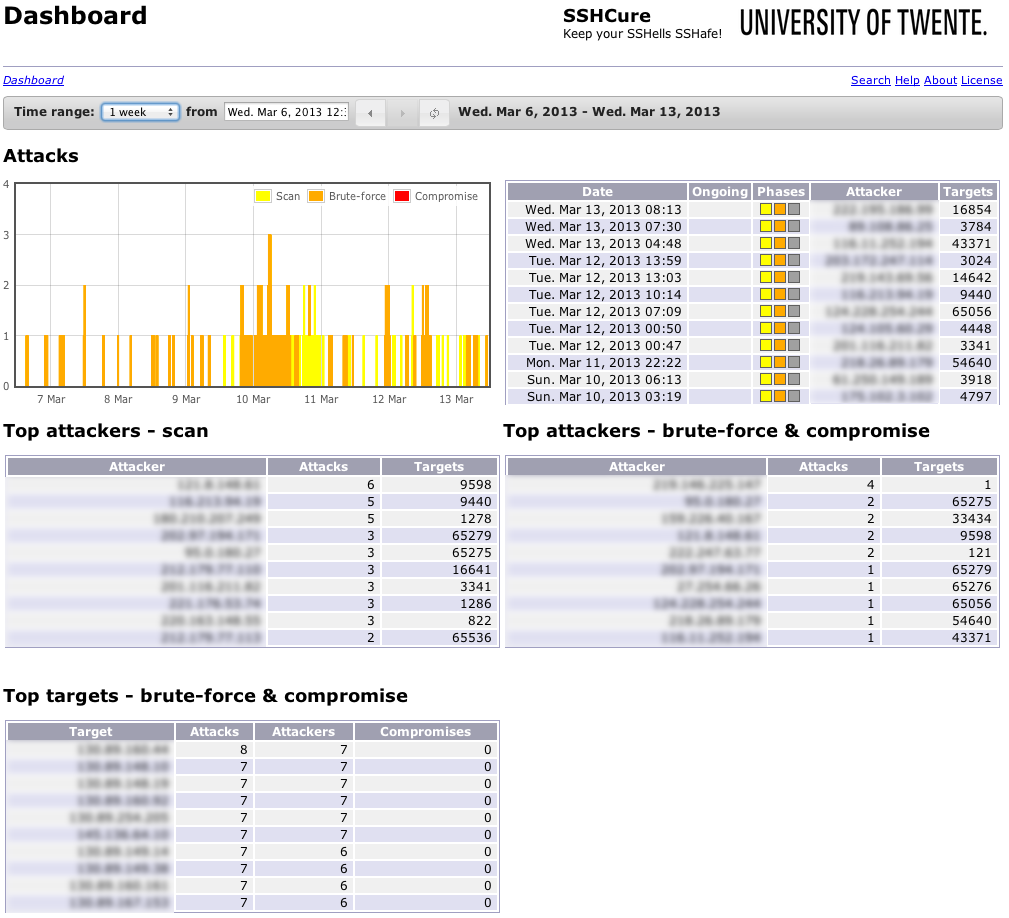
\includegraphics[width=\textwidth]{img/Screenshot_Dashboard_anonymized.png}
	\caption{SSHCure's Dashboard page}
	\label{fig:screenshot_Dashboard}
\end{figure}

At the top of the Dashboard page the time range for the page can be selected. In this screenshot, a time range of `1 week' has been selected. To the right of the time range selector a date/time selector can be found for setting the start of the time range. The following three buttons can be found next to it:

\begin{enumerate}
	\item Back -- Navigate backwards in time by the selected time range -- in the case of the screenshot `1 week'.
	\item Forward -- Navigate forward in time by the selected time range. That button has been disabled in this screenshot, as it is not possible to navigate into the future.
	\item Auto-Refresh / Now -- When the currently selected time range is the latest available, the third button can be used to enabled 'auto-refresh-'. This will update your Dashboard every five minutes, as new data becomes available to NfSen. If the currently selected time range is in the past, the last button can be used to forward to 'now'.
\end{enumerate}

The top left of the Dashboard page shows an attack history plot, where the number of attacks per attack type is shown for the selected time range. Next to it is a list of all attacks that shows all attacks during that occurred during the selected time range. The remaining lists shows statistics for the top scan attackers, top brute-force and compromise attackers and top targets.

\newpage

\begin{figure}[!ht]
	\centering
    	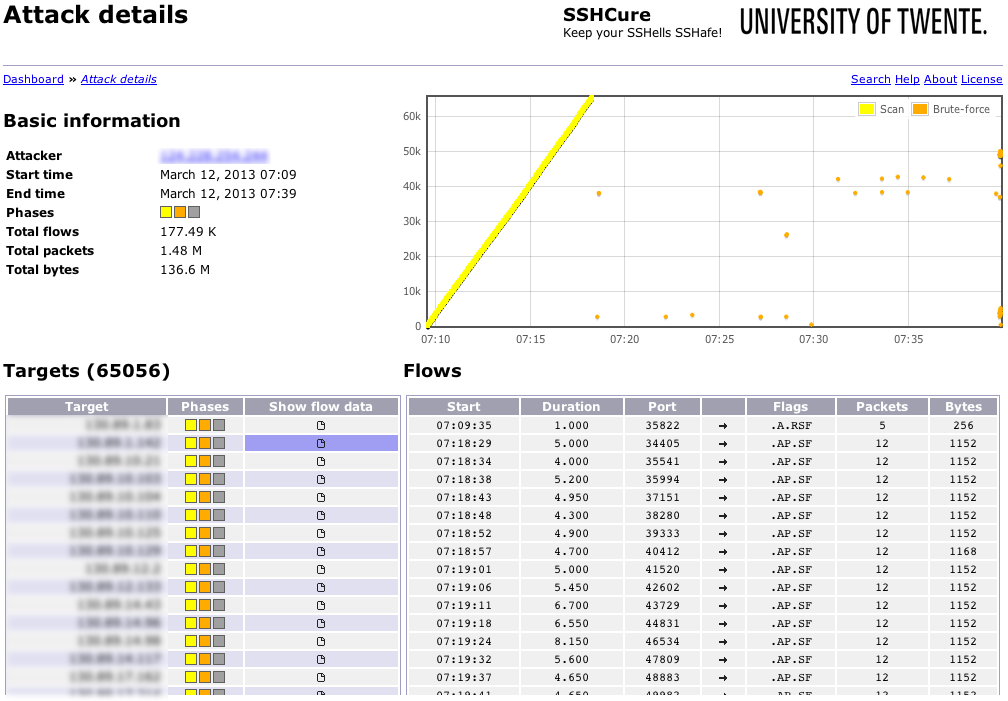
\includegraphics[width=\textwidth]{img/Screenshot_AttackDetails_anonymized.png}
	\caption{SSHCure's Attack Details page}
	\label{fig:screenshot_AttackDetails}
\end{figure}

The top left of the Attack Details page shows basic information on the selected attack, such as start and end time, the identified attack phases and statistics on the network traffic that was part of the attack. In the case of the screenshot, the attack consisted of both a scan and brute-force attempts, but no compromise (so the attack was not successful). To the right of the basic information is an attack profile plot, which shows the contacted hosts (y-axis) and the time (x-axis). It can be observed that a horizontal network scan took place from 07:10 -- 07:18, after which several individual hosts have been brute-forced by means of a dictionary attack.

At the bottom of the page a list of targets is shown. For very large attacks, not all attacks are shown\footnote{See Section~\ref{subsec:frontend_configuration} for more details.}. For each of the listed targets the corresponding flow data can be shown to the right of the targets listing. In the case of the screenshot, flow data is shown for the second target.

\newpage

\begin{figure}[!ht]
	\centering
    	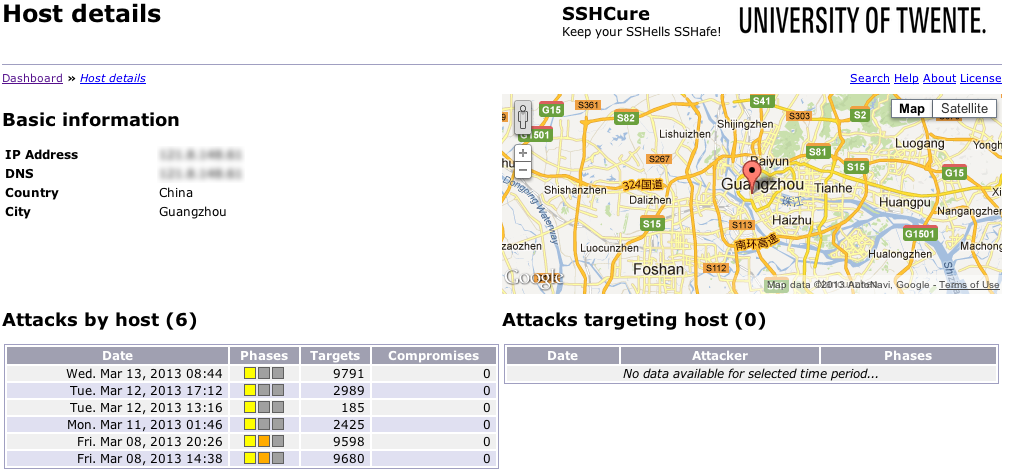
\includegraphics[width=\textwidth]{img/Screenshot_HostDetails_anonymized.png}
	\caption{SSHCure's Host Details page}
	\label{fig:screenshot_HostDetails}
\end{figure}

The third type of page within SSHCure is the Host Details page, which shows specific information on hosts (both attackers and targets). Some basic information, such as IP address, reverse DNS and geolocation information are shown at the top of the page. The bottom of the page consists of two lists: `Attacks by host' and `Attacks targeting hosts'. The first lists all attacks in which the selected host participated as an attacker. The second lists all attacks in which the selected host has been a target.

\cleardoublepage

\section{Troubleshooting \& FAQ}
\label{sec:troubleshooting_faq}

If you encounter any problems with SSHCure, please perform the following steps:

\begin{enumerate}
	\item Make sure to run SSHCure from within NfSen, instead of as a standalone application. This means that you have to run SSHCure from the \emph{Plugins} tab in NfSen.
	
	\item When loading SSHCure, it performs numerous checks in the backend. If any problem has been detected, a warning will be shown at the top of the Dashboard page.
	
	\item Clear the cache of your Web browser.
\end{enumerate}

Despite the fact that SSHCure has been developed with great care, you might encounter errors and/or find bugs. It could also be possible that you have ideas for improvement of SSHCure. Please help us improving SSHCure by sending an e-mail. Last but not least, we are happy to help you configuring SSHCure for use in your environment.

\vspace{3mm}
E-mail: \url{r.j.hofstede@utwente.nl}
\vspace{3mm}
	
Please do always provide as much information and details as possible when making a support request. Your support is honestly appreciated!

\subsection{Profiling}

SSHCure maintains a `profiling database' with anonymous statistics on its performance. You can check out its contents yourselves as follows:

{\tt\small
\begin{verbatim}
$ printf ".header on\n.mode column\n select * from profile;" 
                | sqlite3 /data/nfsen/plugins/SSHCure/data/SSHCure_profile.sqlite3

time        db_size   run_time    target_count_scan  target_count_bf  target_count_do  maintenance_failed
----------  --------  ----------  -----------------  ---------------  ---------------  ------------------
1364198400  500       25          4000000            1000             3                0                 

\end{verbatim}
}

The following parameters are stored in the `profile' table of the database:

\begin{description}
	\item [time] -- UNIX timestamp of the moment in which the record has been created.
	
	\item [db\_size] -- Size of the SSHCure database (\textit{SSHCure.sqlite3}) in bytes.
	
	\item [run\_time] -- Processing time of the SSHCure backend (every five minutes) in seconds.
	
	\item [target\_count\_scan] -- Number of scan targets in the SSHCure database.
	
	\item [target\_count\_bf] -- Number of brute-force targets in the SSHCure database.
	
	\item [target\_count\_do] -- Number of die-off targets in the SSHCure database.
	
	\item [maintenance\_failed] -- Indicates whether a database maintenance run has failed (\textsc{1}) or not (\textsc{0}). A reason for a run to fail can be that the processing time of the SSHCure backend is too long (see `run\_time').
	
	\item [ignored\_records\_close\_outlier] -- Number of flow records within the current \textit{nfdump} file that have starting times within a 24 hour window of the \textit{nfdump} file timestamp, but are still clear outliers with respect to the current \textit{nfdump} file. These flow records are ignored in the intrusion detection process.
	
	\item [ignored\_records\_far\_outlier] -- Number of flow records within the current \textit{nfdump} file that have starting times outside a 24 hour window of the \textit{nfdump} file timestamp. These flow records are ignored in the intrusion detection process.
\end{description}

As the profiling database maintained by SSHCure contains solely anonymous usage statistics, we'd like to ask you to send\footnote{You can find the contact information at the top of this page.} it to us periodically. This will help us to optimize SSHCure for deployment in a wider range of systems/setups.

\subsection{Run lock}

SSHCure uses a `run lock' mechanism as of version 2.0. This means that if the SSHCure backend is executed while the previous execution has not yet completed, backend execution is skipped. This particular event is written to syslog as follows:

\begin{center}
\textit{SSHCure: Previous run has not finished yet (or a stale lock file exists); skipping data processing...}
\end{center}

The `run lock' is stored in the \textit{/data/} directory of SSHCure's backend, together with the database files. In case you suspect that for whatever reason the `run lock' has not been successfully deleted, you can remove the \textit{run.lock} file.

\subsection{Network traffic from SSHCure backend: Version check}

As of version 2.2, SSHCure's backend performs a version check on initialization (i.e., when the NfSen daemon is started). As such, an HTTP POST message is sent out to retrieve the latest version. In case you find SSHCure generating an outbound connection, this is the reason. SSHCure is able to deal with HTTP(S) proxies, configured by means of environment variables.

\cleardoublepage

\section*{License}
\label{sec:license}

The SSHCure project is distributed under the BSD license:

\vspace{2 mm}

\noindent
Copyright (c) 2014, Luuk Hendriks, Rick Hofstede (University of Twente, The Netherlands) \\
All rights reserved. \\

\noindent
Redistribution and use in source and binary forms, with or without modification, are permitted provided that the following conditions are met:

\begin{itemize}
	\item Redistributions of source code must retain the above 
		copyright notice, this list of conditions and the following 
		disclaimer.
	\item Redistributions in binary form must reproduce the above 
		copyright notice, this list of conditions and the following 
		disclaimer in the documentation and/or other materials 
		provided with the distribution.
	\item Neither the name of the University of Twente, nor the
		names of its contributors may be used to endorse or
		promote products derived from this software without
		specific prior written permission.
\end{itemize}

THIS SOFTWARE IS PROVIDED BY THE COPYRIGHT HOLDERS AND CONTRIBUTORS "AS IS" AND ANY EXPRESS OR IMPLIED WARRANTIES, INCLUDING, BUT NOT LIMITED TO, THE IMPLIED WARRANTIES OF MERCHANTABILITY AND FITNESS FOR A PARTICULAR PURPOSE ARE DISCLAIMED. IN NO EVENT SHALL THE COPYRIGHT OWNER OR CONTRIBUTORS BE LIABLE FOR ANY DIRECT, INDIRECT, INCIDENTAL, SPECIAL, EXEMPLARY, OR CONSEQUENTIAL DAMAGES (INCLUDING, BUT NOT LIMITED TO, PROCUREMENT OF SUBSTITUTE GOODS OR SERVICES; LOSS OF USE, DATA, OR PROFITS; OR BUSINESS INTERRUPTION) HOWEVER CAUSED AND ON ANY THEORY OF LIABILITY, WHETHER IN CONTRACT, STRICT LIABILITY, OR TORT (INCLUDING NEGLIGENCE OR OTHERWISE) ARISING IN ANY WAY OUT OF THE USE OF THIS SOFTWARE, EVEN IF ADVISED OF THE POSSIBILITY OF SUCH DAMAGE.


\section*{Acknowledgements}
This work has been supported by SURFnet's GigaPort 3 project on Next-Generation Networks and FLAMINGO, a Network of Excellence 
project (ICT-318488) supported by the European Commission under its Seventh Framework Programme.

\newpage
\bibliographystyle{ieeetr}
\bibliography{sshcure}

\label{totalpages}	% label to count total number of pages in your document, please don't remove it
\end{document}
